% \iffalse
\let\negmedspace\undefined
\let\negthickspace\undefined
\documentclass[journal,12pt,twocolumn]{IEEEtran}
\usepackage{cite}
\usepackage{amsmath,amssymb,amsfonts,amsthm}
\usepackage{algorithmic}
\usepackage{graphicx}
\usepackage{textcomp}
\usepackage{xcolor}
\usepackage{txfonts}
\usepackage{listings}
\usepackage{enumitem}
\usepackage{mathtools}
\usepackage{gensymb}
\usepackage{comment}
\usepackage[breaklinks=true]{hyperref}
\usepackage{tkz-euclide} 
\usepackage{listings}
\usepackage{gvv}                                        
\def\inputGnumericTable{}                                
\usepackage[latin1]{inputenc}                            
\usepackage{color}                                       
\usepackage{array}                                       
\usepackage{longtable}                                   
\usepackage{calc}                                        
\usepackage{multirow}                                    
\usepackage{hhline}                                      
\usepackage{ifthen}                                      
\usepackage{lscape}
\usepackage{amsmath}
\newtheorem{theorem}{Theorem}[section]
\newtheorem{problem}{Problem}
\newtheorem{proposition}{Proposition}[section]
\newtheorem{lemma}{Lemma}[section]
\newtheorem{corollary}[theorem]{Corollary}
\newtheorem{example}{Example}[section]
\newtheorem{definition}[problem]{Definition}
\newcommand{\BEQA}{\begin{eqnarray}}
\newcommand{\EEQA}{\end{eqnarray}}
\newcommand{\define}{\stackrel{\triangle}{=}}
\theoremstyle{remark}
\newtheorem{rem}{Remark}
\graphicspath{{./figs/}}

\begin{document}

\bibliographystyle{IEEEtran}
\vspace{3cm}

\title{NCERT Mathematics Ex 9.4 Q6}
\author{EE23BTECH11059 - Tejas$^{}$% <-this % stops a space
}
\maketitle
\newpage
\textbf{Question:}
1) Find the sum to n terms of\\$3 \times 8 + 6 \times 11 + 9 \times 14 + ...$
    \solution
        Writing the general term of the series
        \begin{align}
            x\brak{n}&=\brak{3n+3}\brak{8+3n}u\brak{n}
        \end{align}
        The sum of n terms of this progression can be given by:
        \begin{align}
            y\brak{n} &= x\brak{n}*u\brak{n}\\
            \implies  Y\brak{z} &= X\brak{z}U\brak{z} \label{eq:eq3}
        \end{align}
        $z$ transform of $x\brak{n}$:
        \begin{align}
            X\brak{z} &= \sum_{n=0}^{\infty} \brak{3n+3}\brak{3n+8}z^{-n} \\
            X\brak{z} &= \sum_{n=0}^{\infty} \brak{9n^2 +33n+24}z^{-n} \\
            X\brak{z}&=9z^{-1}\frac{\brak{1+z^{-1}}}{\brak{1-z^{-1}}^3} + \frac{33}{\brak{1-z^{-1}}^2} +\frac{24}{\brak{1-z^{-1}}}; \abs{z}>1    \label{eq:eq5}
        \end{align}
        Using equation \eqref{eq:eq5} and equation \eqref{eq:eq3} we get Y\brak{z} as:
        \begin{align}
            Y\brak{z}&= \frac{\brak{z}^{-1}\brak{18-9z^2+67}}{\brak{1-z^{-1}}^3} + \frac{\brak{42-9z^{-1}}}{\brak{1-z^{-1}}^2} 
        \end{align}
        \begin{align}
            nu\brak{n} &\system{Z} \frac{z^{-1}}{\brak{1-z^{-1}}^2} \cbrak{\abs{z}>1} \label{eq:z transform of nu{n}} \\
            n^2 u\brak{n} &\system{Z} \frac{z^{-1}\brak{1+z^{-1}}}{\brak{1-z^{-1}}^3} \cbrak{\abs{z}>1}\label{eq:z transform of n^2u{n}} \\
            n^3 u\brak{n} &\system{Z} \frac{z^{-1}\brak{1+4z^{-1}+z^{-2}}}{\brak{1-z^{-1}}^4} \cbrak{\abs{z}>1}\label{eq:z transform of n^3u{n}} 
        \end{align}
        \begin{align}
            n^4 u{n} &\system{Z} \frac{z^{-1}\brak{1+11z^{-1}+11z^{-2}+z^{-3}}}{\brak{1-z^{-1}}^5} \cbrak{\abs{z}>1}\label{eq:z transform of n^4u{n}}
        \end{align}
        Taking reverse z transform, using equations \eqref{eq:z transform of nu{n}} to \eqref{eq:z transform of n^4u{n}}
        We get $y\brak{n}$ as: 
        \begin{align}
            y\brak{n}=\frac{33n\brak{n+1}}{2}+\frac{9n\brak{n+1}\brak{2n+1}}{6}+24\brak{n+1}
        \end{align}
        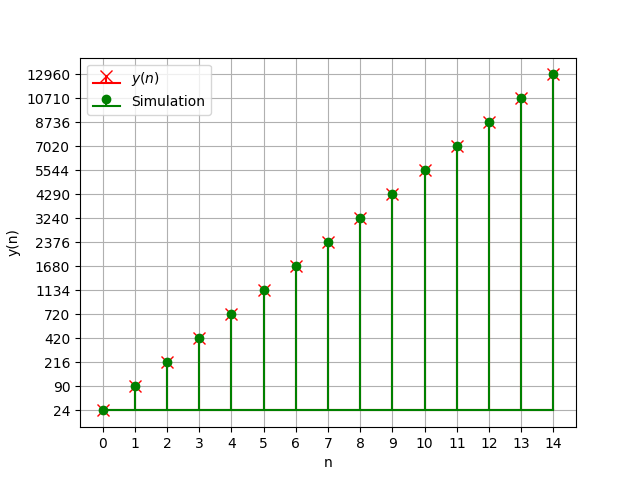
\includegraphics[width=\columnwidth]{figs/plot.png}
        \label{fig:Graph1_math.11.9.4.8}
\renewcommand{\thefigure}{\theenumi}
\renewcommand{\thetable}{\theenumi}
\end{document}
